\section{Standard Machine Learning Methods}
\label{appendix:ML_methods}
\subsection{Principal Component Analysis (PCA)}
\label{sec:methods:pca}
PCA \cite{wold_principal_nodate} is a dimensionality reduction technique which aims to project high-dimensional data into a new, more meaningful basis by re-expressing the data through a linear combination of these new basis vectors. This linearity allows us to pose the problem through linear algebra, where we wish to find a linear transformation $\boldsymbol{P}$ which maps the original recorded dataset $\bf X$ to a new representation of that dataset $\boldsymbol{Y}$ such that:
\begin{equation}
    \boldsymbol{Y} = \boldsymbol{P} \cdot \boldsymbol{X}.
\end{equation}
The rows of $\boldsymbol{P}$ then form a new set of orthonormal basis vectors. To find $\bf P$, we assume that axes of interest are those with high variance. These high variance axes can be found by calculating the eigenvectors of the covariance matrix of the dataset: 
\begin{equation}
    \boldsymbol{C} = \frac{1}{n} \boldsymbol{X} \boldsymbol{X}^T,
\end{equation}
which itself gives the degree of linear relationship between different variables. The eigenvalues of $\boldsymbol{C}$ therefore correspond to the variance of $\boldsymbol{X}$ along the associated eigenvector \cite{shlens_tutorial_2014}. Throughout this work, PCA is used to reduce inputs to 25 dimensions.

\subsection{Linear Discriminant Analysis (LDA)}
\label{sec:methods:lda}
LDA \cite{fisher_use_1936} is a classification technique which aims to maximise the separability of classifications for given input data (e.g. IR spectra) by maximising between-class variance and minimising within-class variance \cite{tharwat_linear_2017}. This is achieved by assuming data corresponding to a specific class $k$ is normally distributed about a mean value $\mu_k$, and that all classes have equal covariance matrices $\boldsymbol{\Sigma}_k=\boldsymbol{\Sigma}$. The first assumption requires there to be a point $x^*$ which is equally likely to belong to two classes. If we take $x^*$ as the decision boundary, we can then minimise the classification error, which in the binary classification case with classes $\mathcal C_1$ and $\mathcal C_2$ is given by:
\begin{equation}
   \mathbb{P}(\text{error})= \mathbb{P}(x>x^*, x\in \mathcal C_1) + \mathbb{P}(x<x^*, x\in \mathcal C_2).
\end{equation}
Minimising this error with respect to $x^*$, denoting the probability density within each class as $f_k(x)$ and denoting priors for each class by $\pi_k$ then gives;
\begin{equation}
    f_1(x^*)\pi_1 = f_2(x^*)\pi_2.
\end{equation}
Now considering multi-class classification and assuming the data follows a multivariate Gaussian distribution of dimension $d$, we have;
\begin{equation}
    f_k(\boldsymbol{x})\pi_k=\frac{1}{\sqrt{(2\pi)^{d}|\mathbf{\Sigma}_k|}}\exp\left(-\frac{1}{2}(\boldsymbol{x}-\boldsymbol{\mu}_k)^T\boldsymbol{\Sigma}_k^{-1}(\boldsymbol{x}-\boldsymbol{\mu}_k)\right)\pi_k.
\end{equation}
Taking the logarithm of this, discounting constant terms and enforcing the equal covariance assumption gives scaled posterior probabilities for each class $k$ as:
\begin{equation}
    \delta_k(\boldsymbol{x}) = \boldsymbol{\mu}_k^T\boldsymbol{\Sigma}^{-1}\boldsymbol{x} - \frac{1}{2}\boldsymbol{\mu}_k^T\boldsymbol{\Sigma}^{-1}\boldsymbol{\mu}_k + \ln(\pi_k).
\end{equation}
The classification $k$ with maximal $\delta_k(\boldsymbol{x})$ is then chosen as the predicted class for $\boldsymbol{x}$ \cite{ghojogh_linear_2019}. In practice, the priors $\pi_k$ are estimated according to the proportion of samples in each class, and the means $\boldsymbol \mu_k$ and covariance matrices $\boldsymbol{\Sigma_k}$ are estimated using maximum likelihood estimation (MLE) \cite{haynes_maximum_2013}. In the mean case, this is given by:
\begin{equation}
    \boldsymbol{\mu}_k = \frac{1}{n_k}\sum_{i=1}^{n}\boldsymbol{x}_i \mathbb{I}(\mathcal C(\boldsymbol x_i)=k),
\end{equation}
where $\mathbb{I}$ is the indicator function \cite{ghojogh_linear_2019}. As we assume the covariance matrices are the same for each class, we take $\boldsymbol \Sigma$ to be the weighted sum of the estimated covariance matrices for each class. This can be considered geometrically \cite{mika_fisher_1999,tharwat_linear_2017} by solving an eigenvalue problem as is shown in Figure \ref{fig:LDA}. New data can then be classified by finding the projected training class mean which minimises the distance to the projection of test data within the eigenvector space.

\begin{figure}[htbp]
  \centering
  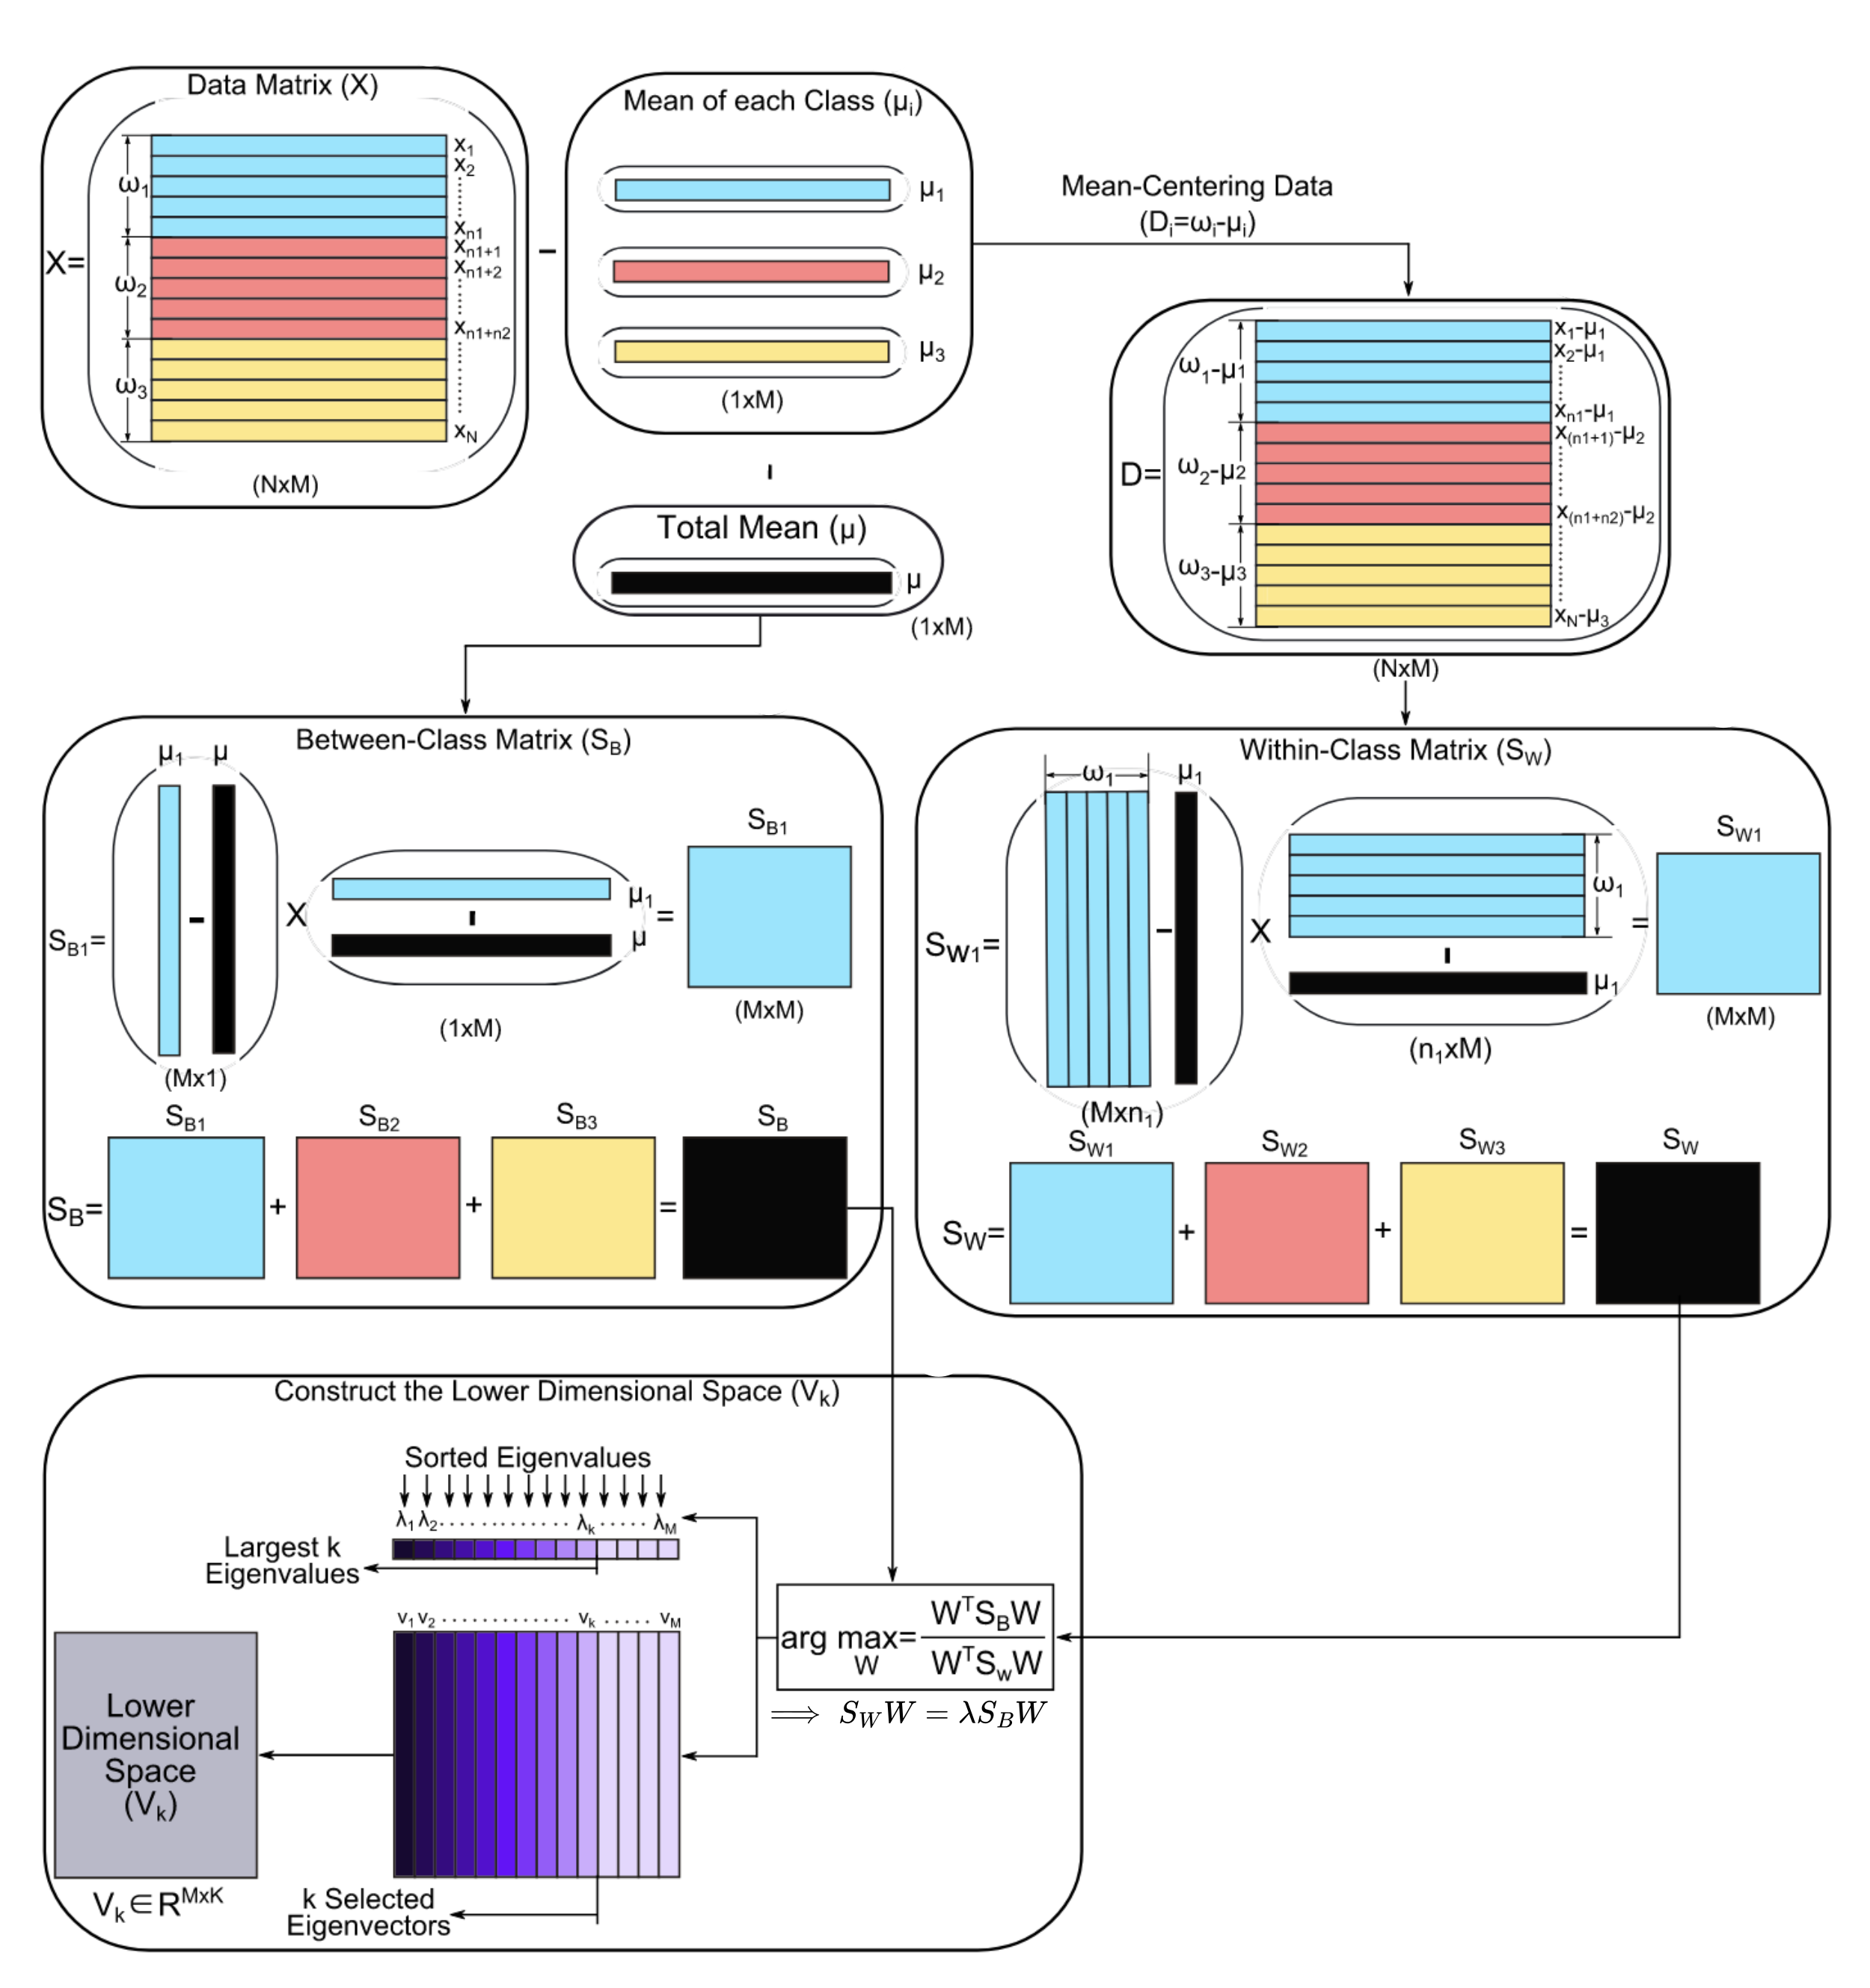
\includegraphics[width=1\textwidth]{Images/LDA.png}
  \caption{A graphical representation of the LDA algorithm. Each class $\omega_k$ is coloured differently. Note the use of Fisher's criterion in the lowest cell which is rewritten in eigen-equation form; $S_W W=\lambda S_B W$. Modified from  \cite{tharwat_linear_2017}.}
  \label{fig:LDA}
\end{figure}



\subsection{Extreme Gradient Boosting (XGBoost or XGB)}
\label{sec:methods:xgboost}
XGBoost generates an ensemble of regression T-trees (trees with T leaves) - producing $K$ additive functions $f_k$, which combined, learn to map inputs to continuous values
\begin{equation}
    \hat y_i = \sum_{k=1}^K f_k(\boldsymbol{x}_i),
\end{equation}
subject to the regularisation objective
\begin{equation}
    \mathcal L (\phi)= \sum_i l(\hat y_i, y_i)+\sum_k\Omega(f_k).
\end{equation}
Here, $l$ is a differentiable loss between the prediction $\hat y_i$ and target value $y_i$, and $\Omega(f)$ is a complexity penalising regularisation term \cite{chen_xgboost_2016}. We assemble the ensemble of trees iteratively. At each iteration, $t$, we add $f_t$ to the prediction at the previous iteration and minimise
\begin{align}
    \mathcal L^{(t)}&=\sum_{i=1}^nl(y_i, \hat y_i^{(t-1)}+f_t(\boldsymbol{x}_i))+\Omega(f_t)\\
    &\approx \sum_{i=1}^n \left[l(y_i, \hat y^{(t-1)})+g_i f_t (\boldsymbol{x}_i)+\frac{1}{2} h_if_t^2(\boldsymbol{x}_i)\right]+\Omega(f_t),
\end{align}
where $g_i=\partial_{\hat y^{(t-1)}} l(y_i, \hat y^{(t-1)})$ and $h_i=\partial^2_{\hat y^{(t-1)}}l(y_i, \hat y^{(t-1)})$ are first and second order gradients of the loss function \cite{friedman_additive_2000}. Minimising this loss over a leaf then gives the optimal tree weighting 
$w_j$ for that leaf. Many further optimisation techniques are used to improve the performance of XGBoost, the details of which can be found in \cite{chen_xgboost_2016}. A final prediction is then made by summing contributions from each tree for a given input, as shown in Figure \ref{fig:tree_ensemble}. Note that for $N$-classification tasks, $N$ trees - corresponding to positive and negative classification for each class - are built at each iteration, with softmax \cite{bridle_probabilistic_1990} over the summed outputs from these trees used to select the best classification.

\begin{figure}[htbp]
  \centering
  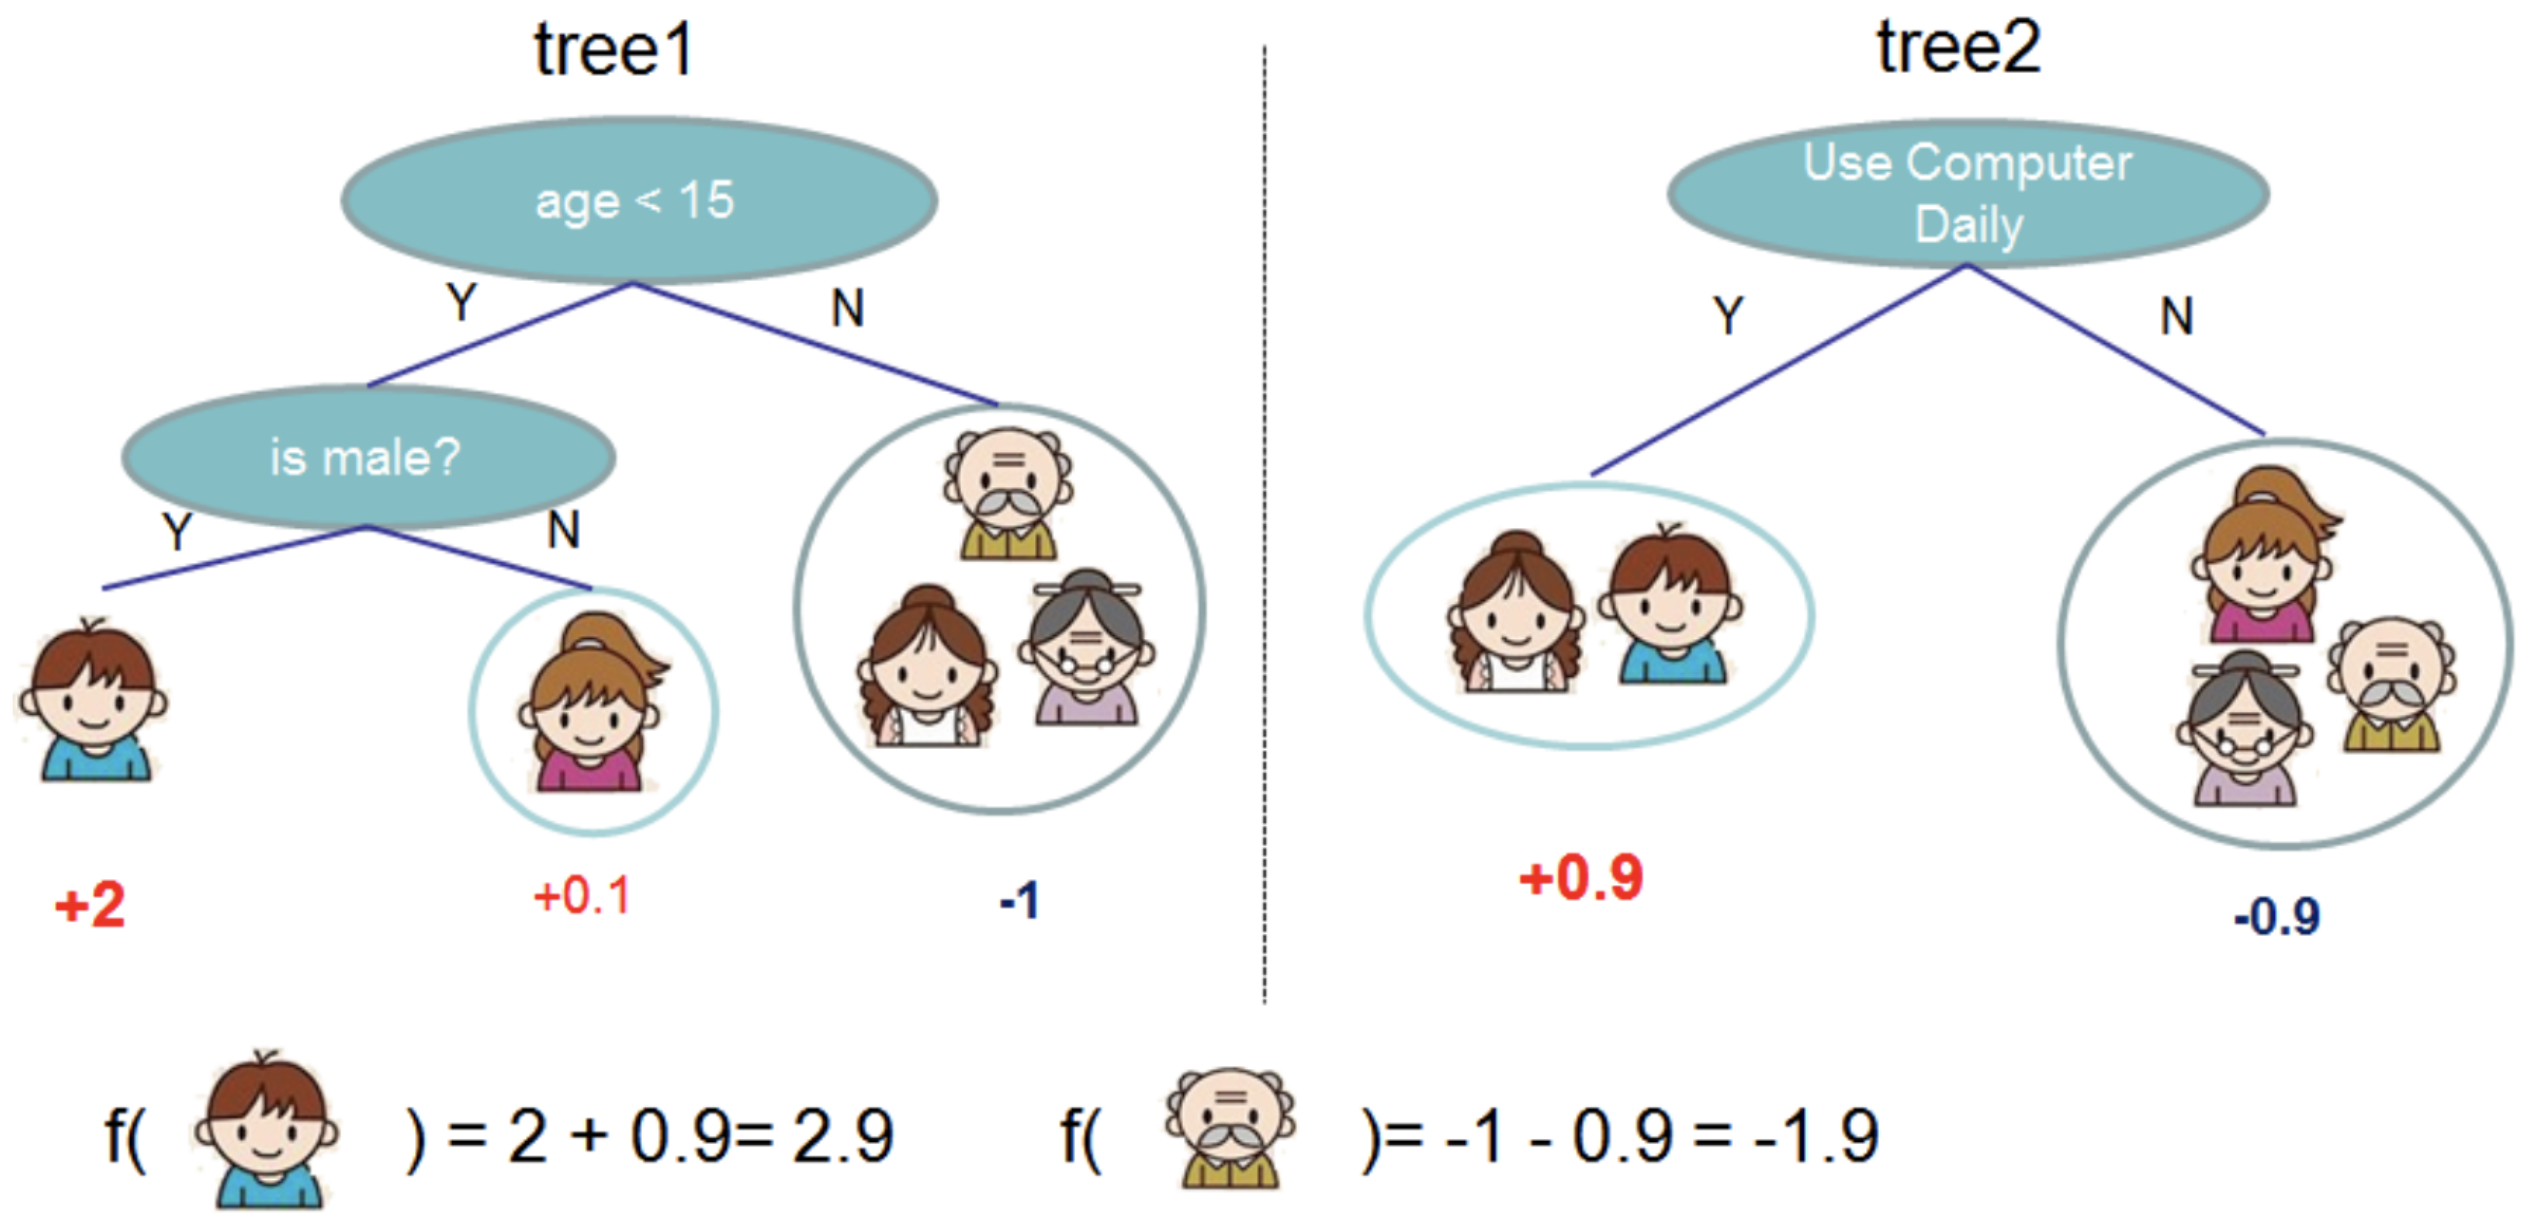
\includegraphics[width=0.8\textwidth]{Images/tree_ensemble.png}
  \caption{A tree ensemble model, where final predictions are the sum of those from each tree. From \cite{chen_xgboost_2016}.}
  \label{fig:tree_ensemble}
\end{figure}